\begin{opin}{\guscolor}{Gustavo}

\subsubsection{Divulgación de las Matemáticas como docentes}

En la clase de hoy Raquel hizo referencia a un debate que puede generar polémica. El asunto es si las matemáticas son asequibles para todo el mundo o solo para elegidos como algunos piensan. Raquel es partidaria de que todo el mundo podría aprender matemáticas correctamente si estas se explican cómo deberían. En mi opinión, yo no afirmaría ni una cosa ni la otra al 100\%, es decir, no todo es blanco ni negro. Relacionándolo con las inteligencias múltiples que explicó Helena López Casares en la conferencia que dio el 20 de septiembre en el Campus Vicálvaro, me atrevería a decir que un profesor puede intentar despertar el interés de un alumno por las matemáticas, pero es cierto que dentro de todas las posibles inteligencias que pueden existir, si un alumno no tiene bien desarrollada la inteligencia relacionada con las matemáticas, un profesor podrá ser capaz de despertasr el interés de un alumno hasta un límite.

En cualquier caso, ya sea para difundir las matemáticas a todo el mundo o no, lo que está claro es que hay que intentar quitar ese estigma existente dentro del mundo matemático acerca de que la gente a la que le gustan las matemáticas son “bichos raros”. Para ello hay que difundir y divulgar las matemáticas y qué mejor manera que hacerlo de un tiempo a esta parte que a través de la prensa y de los medios de comunicación. 

El problema está en que los periodistas históricamente han huido de las matemáticas desde bien entrada la Universidad y por tanto existen muchos errores en prensa y televisión acerca de las matemáticas como se pueden ver en las transparencias de clase o en el video visto en clase de Marilo Montero (https://www.youtube.com/watch?v=zclITKd4ivQ). Este error tiene que ver con el error o fallo que puede existir a la hora de representar ciertas expresiones matemáticas como puede ser la expresión 48/2(9+3) y que ha generado un debate en los foros de la asignatura que muestro a continuación dado que  me pareció muy interesante y no tuvimos tiempo para abordarlo en clase

En mi opinión, inicialmente el resultado era 2, clarísimamente. Pero después de razonar con mis compañeros de clase vi que podría haber más soluciones aparte de la mia. David Soria explicó lo siguiente: 

\begin{mdframed}
El problema tiene dos opciones distintas dependiendo del orden de operación. Hay dos elementos de distinto orden que son PEMDAS Y BEDMAS, según en la escuela que te hayan enseñado puede ser uno u otro. El orden para aplicar las operaciones en PEMDAS (Paréntesis, Eponenciación, Multiplicación, División, Adición y Sustracción) mientras que el orden en BEDMAS (Paréntesis,, Exponenciación, División, Multiplicación, Adición y Sustracción). 

Con PEMDAS el resultado de la operación sería 2.

\[
48÷2·(9+3) \to 48 ÷ 2·(12) \to 48÷2·12 \to 48÷24 = 2
\]

Con BEMDAS  el resultado de la operación seria 288.

\[
48÷2·(9+3) \to 48 ÷ 2·(12) \to 24·12 = 288
\]

\end{mdframed}

Antonio Jesus Guerrero y Carlos Rodiño entendían que “que multiplicar y dividir están al mismo nivel, igual que sumar y restar; y que en tal caso la prioridad de operación es de izquierda a derecha.”

Posteriormente, Manuel Pulido compartió su forma de pensar con Carlos y con Antonio,  y además corroboró la información con un libro de texto indicando que es la manera más extendida de hacerlo.

El libro de texto decía lo siguiente:

\textit{En general:}

\begin{itemize}
\item \textit{En operaciones con paréntesis, primero hay que realizar las que están entre paréntesis y luego las demás.}
\item \textit{En operaciones sin paréntesis, primero se efectúan las multiplicaciones y divisiones y luego, las sumas y las restas.}
\item \textit{En operaciones de igual prioridad, primero la de más a la izquierda.}
\end{itemize}

\textit{Por lo tanto ellos lo calcularían así:}

\[
48÷2·(9+3) \to 48 ÷ 2·(12) \to 24·12 = 288
\]



Por último, intenté llegar a una conclusión que es la importancia que tiene como colocar las expresiones matemáticas para no dar lugar a ambigüedades de este estilo.


Lo que queda claro es que unos entienden la expresión como $\frac{48}{2(9+3)}$ y otros como $\frac{48}{2}(9+3)$.

Si ambas expresiones se reflejaran así no daría lugar a ninguna confusión.

En cualquier caso no estoy de acuerdo en aplicar las reglas que indican ciertos libros de texto dado que si aplicamos estas reglas indicadas por el libro de texto al que hacía referencia Manual, la expresión 

Podría interpretarse como si fuera igual a 288, cuando todos tenemos claro que debe ser igual a 2.

Para terminar el debate Miriam Expóstio indicó que 
\textit{Desde mi punto de vista, para que se entendiese que hay que dividir todo entre "2(9+3)" se tendría que poner todo ese término entre corchetes, no?}


Con lo que estoy totalmente de acuerdo. Y por tanto, al no haber corchetes, el problema lo tiene quien escribe la expresión al haber varias interpretaciones.
Las matemáticas deben ser exactas y no dar lugar a interpretaciones. Para interpretaciones ya están las leyes ;-)
Además de los errores cometidos por los periodistas de manera involuntaria como puede ser el de Mariló también están los errores cometidos intencionadamente con el objetivo de manipular a esa parte de la sociedad menos documentada. Ejemplos pueden ser el número de asistentes a una manifestación que varía en función de diversos intereses.
También hablamos acerca de los errores comunes que tienen los alumnos a la hora de realizar ciertas operaciones básicas en matemáticas y que independientemente de ser de letras o de ciencia, no se deberían cometer. Es como si los de ciencia dijeran que no saben escribir gramaticalmente bien porque son de ciencia. No tiene sentido. La cultura es independiente de ser de ciencias o de letras.
Otra de las formas de divulgar las matemáticas en televisión es a través de series. Por ejemplo:

\begin{itemize}
\item “Universo matemático” era una serie, producida en el año 2000, que constaba de 10 capítulos y que abordaba distintos temas relacionados con la matemática. La obra obtuvo en el año 2002 el Premio a la divulgación científica del Festival Internacional Científico de Pekín. 
\item Se puede ver en 
\href{http://www.rtve.es/alacarta/videos/universo-matematico/} {http://www.rtve.es/alacarta/videos/universo-matematico/} 
\item “Más por menos”. Esta serie consta de 13 programas emitidos de septiembre de 1996 a enero de 1997 y de noviembre de 2002 a enero de 2003 en el programa de Televisión Educativa de TVE-2 "La Aventura del Saber".
\item Se puede ver en 
\href{http://www.rtve.es/television/la-aventura-del-saber/documentales/mas-por-menos/} {http://www.rtve.es/television/la-aventura-del-saber/documentales/mas-por-menos/} 
\item “Orbita Laika” sección de Matemáticas por Raúl Ibañez.
\item Matemáticas invisibles:
\begin{itemize}
\item Curiosidad sobre el tamaño de las hojas DINA-n (
\href{http://www.sabercurioso.es/2008/11/05/por-que-una-hoja-de-papel-din-a4-tiene-el-tamano-que-tiene/}{http://www.sabercurioso.es/2008/11/05/por-que-una-hoja-de-papel-din-a4-tiene-el-tamano-que-tiene/}
)
\item Explicación del digito de control de un código de barras. Todo tiene su explicación
\end{itemize}
\end{itemize}



Como vemos, hay muchas formas de divulgar las matemáticas y nosotros como futuros docentes debemos ser parte fundamental en el futuro de esta divulgación, ya sean:

\begin{itemize}
\item Artículos en revistas  
\item Convocatorias de actividades relacionadas con las matemáticas (fotografía, concursos, juegos…)
\item Concesiones de premios (Medalla Fields) 
\item Iniciativas como dar publicidad a los congresos internacionales de matemáticas 
\item Promover jornadas de popularización y divulgación  (“olimpiadas matemáticas”) 
\item Museos (Museo Nacional de Ciencia y tecnología, MUNCYT, antiguo Cosmocaixa)) 
\item Páginas web divulgativas
\item Divulgamat (
\href{http://www.divulgamat.net/}{http://www.divulgamat.net/}
)
\end{itemize}

\begin{minipage}[hbtp]{0.5\linewidth}
	\centering
	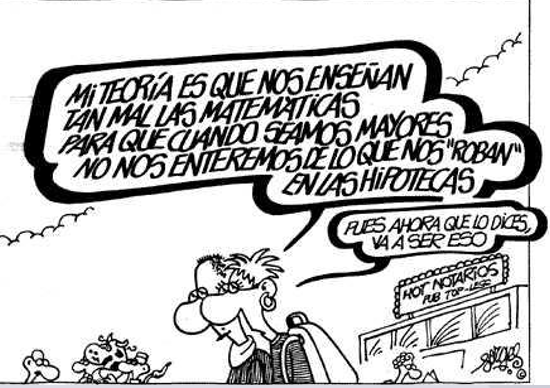
\includegraphics[width=0.8\linewidth]{img/chistegus.png}
	%\captionof{figure}{Coche de mediadios del siglo pasado.}
\end{minipage}

\end{opin}

\begin{opin}{\victorcolor}{Víctor}

En mi diario incluía también una mención sobre el ejemplo $48÷2·(9+3)$ tratado por mi compañero Gustavo, pero lo voy a omitir por evitar repeticiones innecesarias.

\subsubsection{Docentes como divulgadores}

Me ha resultado muy novedosa la idea de que \textit{los profesores deberíamos ser los primeros divulgadores de las Matemáticas} (Antonio Durán). 
%
No sólo en el aula con los alumnos, sino también fuera de ella.
%
Hacen falta personas apasionadas por las Matemáticas, capaces de ayudar a la gente a romper el mito ``Es que soy de letras'' 
%
\footnote{Al igual que personas apasionadas por las letras que rompan con el mito ``Es que soy de ciencias''. Qué pasa, ¿que por ser de ciencias no saber redactar ni expresarte por escrito?}
%
Y a veces, ese argumento se utiliza para escaquearse de llevar las cuentas en un viaje o en una cena, cuyos cálculos no pasan de simples divisiones y sumas que un estudiante de 5º de Primaria podría hacer.

\subsubsection{Construyendo el conocimiento matemático sin lagunas}

En verano estuve de voluntariado en Perú y una semana fue dar clase de mates a chavales de secundaria de allí. 
%
Les ocurría que sabían despejar las ecuaciones perfectamente. Hacían todos los pasos bien, hasta que al llegar al final, $3x = 24 \to x=\frac{24}{3} = ?$. 
%
El último paso no eran capaces de hacerlo. ¿Cómo es posible que lleguen al curso en el que están y sepan despejar sin saberse las tablas de multiplicar? 
%
¡Qué sistema educativo tan ineficiente! 
%
Pasan de curso sin los conocimientos necesarios... construyen el conocimiento con unas lagunas bestiales.

Viendo los errores de primero de grado propuestos por Raquel me doy cuenta que no hay tanta diferencia entre el modelo de allí, con el modelo de aquí; 
%
en cuanto a construir un conocimiento sólido sin lagunas.


La Ted Talk de Salman Khan me parece una charla que todo docente de Matemáticas debería ver (tanto es así, que mi primera aportación a los foros de la asignatura fue plantear esta charla).
%
¿Te imaginas construir el tejado de un edificio sin haber terminado los cimientos?
%
Nadie trabaja así. Ni siquiera nadie, exceptuando a Fito y Fitipaldis, sugiere trabajar así.
%
¿Porqué en Matemáticas enseñamos a integrar sin que se haya interiorizado bien la derivada? ¿Porqué tratamos de enseñar diagonalizar matrices sin que los alumnos tengan claro cómo se factoriza un polinomio con Ruffini?
%
No digo que haya que enseñar Ruffini en la universidad, sino que los docentes en la secundaria nos esforcemos por no dejar lagunas en el conocimiento de los alumnos. 
%
``Enseñar para la maestría'', como dice Salman Khan.

\paragraph{Khan Academy}

Al hilo de retomar esta charla este curso (ya la conocía anteriormente) estuve paseando por la web y viendo los recursos que tienen.
%
Es una pena que esté en inglés y tal vez no sea utilizable en clase, pero ayuda a hacerse una idea de cómo funcionar. 
%
Además, están trabajando en traducciones, para hacer llegar la academia a más países.

Otro aprendizaje, al hilo de Khan, es la importancia del inglés. 
%
Más allá de poder comunicarse, en internet hay infinidad de recursos (empezando por las charlas Ted) que merecen mucho la pena y que se podrían estar aprovechando mucho más, si supiéramos inglés.
%
A raíz de esto, cuando me preguntan qué es lo que más valoro del inglés, lo que siempre contesto es: ``poder aprender autodidactamente de lo que sea en internet y acceder a reflexiones y conocimiento de otras personas''.


\end{opin}

\begin{opin}{\pedrocolor}{Pedro}

.


\end{opin}

\begin{opin}{\virgicolor}{Virginia}
.


\end{opin}
